\chapter{Machine Learning in Physical Investigations}\label{sec:ml}
In the previous chapter, we began with the goal of translating
microscopics to macroscopics. Where MFT failed, RG made sense of
critical phenomena, revealing universality, simple scaling laws,
critical exponents, and relations between them. In this chapter, we
turn to machine learning.  Like RG, ML is a blanket term that refers
to a wide range of techniques. Both involve the iterative manipulation
of information with the goal of extracting ``relevant''
information. However, we will see that ML is more flexible in its
definition of relevant. Whereas in statistical physics, relevant is
synonymous with long-distance, in ML, relevance will depend on the
problem at hand. We will also see that the level at which RG and ML
manipulate information is different. Where statistical physics works
with partition functions, ML works with probabilities. In practice,
many of the challenges (namely, intractable sums), but also solutions,
are the same. In spirit, however, this distinction reveals something
fundamental about the types of challenges that characterize physics
and ML\@.

In physics, our investigations are largely reductionist: we
\textit{begin} with a Hamiltonian, which, in turn, defines a partition
function, and our aim is to predict something about large sets of
microstates. To this end, computational techniques, like MCMC
algorithms, may use $P(\bs)$ (more precisely, the relative
probability) to generate a finite set of samples $\mcS_{data}$ that,
we hope, is representative of $\mcS$, the true, complete set of
microstates. By this, we mean that the statistical properties of
$\mcS_{data}$ and $\mcS$ should converge as we increase the number of
samples. In ML, the investigation often works in the opposite
direction: we are given some $\mcS_{data}$ and assume it is
representative of $\mcS$. Then, our goal is to learn something about
$P(\bs)$. While physics concerns properties of $\mcS$, ML concerns
properties of $\bs$. These are not absolute distinctions, but it will
be valuable to bear in mind.

Let us introduce some of the essentials of ML and show its value for
statistical physics through a practical example. We follow the
treatment of Hinton~\cite{hinton} as well as Mehta et al.'s \textit{A high-bias, low-variance
  introduction to Machine Learning for
  physicists}~\cite{mehta-review}. We refer the interested reader to
these sources for elaboration where our analysis goes quickly.

\section{Phase Classification}
Our first question, as physicists, is the following: can we train a
neural network to classify the likely phase of some Ising
configuration, $\bx$? This immediately reflects the different spirits
of ML and physics we discussed above: our goal is to learn something
about the microstate $\bs$, whereas in the previous chapter we cared
only for $\mcS$. Formally, our aim is to learn the conditional
probability distribution $P(\by|\bx)$, where $\by$ encodes the phase.

We start with a dataset. In this case, we assume we have access to a
large collection of Ising configurations at different temperatures and
phases, $\mcX_{data}\eqcolon\{\bx \}$, as well as their phase labels
$\mcY_{data}\eqcolon\{\by\}$. We often distinguish two kinds of ML\@:
\textit{supervised} and \textit{unsupervised} learning.\footnote{A
  third axis of differentiation, reinforcement learning is outside the
  scope of this capstone.} Our access to labels, $\mc{Y}$, means this
example of classification falls under supervised learning.\footnote{We
  could, however, also formulate classification of phases as an
  unsupervised learning problem. We might try ``clustering,'' where we
  specify a number of clusters, $k$, and try to group training
  examples into as many clusters, according to some notion of
  similarity. Then, we hope that the clusters our model learns
  correspond to the phases. We could also use this procedure with
  different choices of $k$ to determine a likely number of phases.} In
contrast, unsupervised learning works without labels, typically at the
level of $P(\bx)$, detecting patterns in the raw data itself.

Before doing anything else, we randomly divide $\mcX_{data}$'s
elements into a training set, $\mcX_{train}$, from which our network
learns, and a testing set, $\mcX_{test}$, on which we test the trained
model's results. This division is crucial because, in ML, we want our
results to generalize to new samples that may not have been in our
dataset $\mcX_{data}$ but that could have come from $\mcX_{true}$. A
central problem in ML is the \textit{bias-variance tradeoff}. An
algorithm may \textit{overfit} the training set which compromises its
ability to generalize to new data, or it might fail to learn enough
detail, performing poorly on both training and testing data
(low-bias/high-variance and high-bias/low-variance, respectively). By
splitting the dataset into a testing and training set, we get a good
impression of the bias and variance for the models we trained. Often,
we will further split the training set into cross-validation sets,
trying out different kinds of models, ultimately keeping those that
best accomplish a balance of low bias and variance.

\begin{figure}[ht]
  \centering
  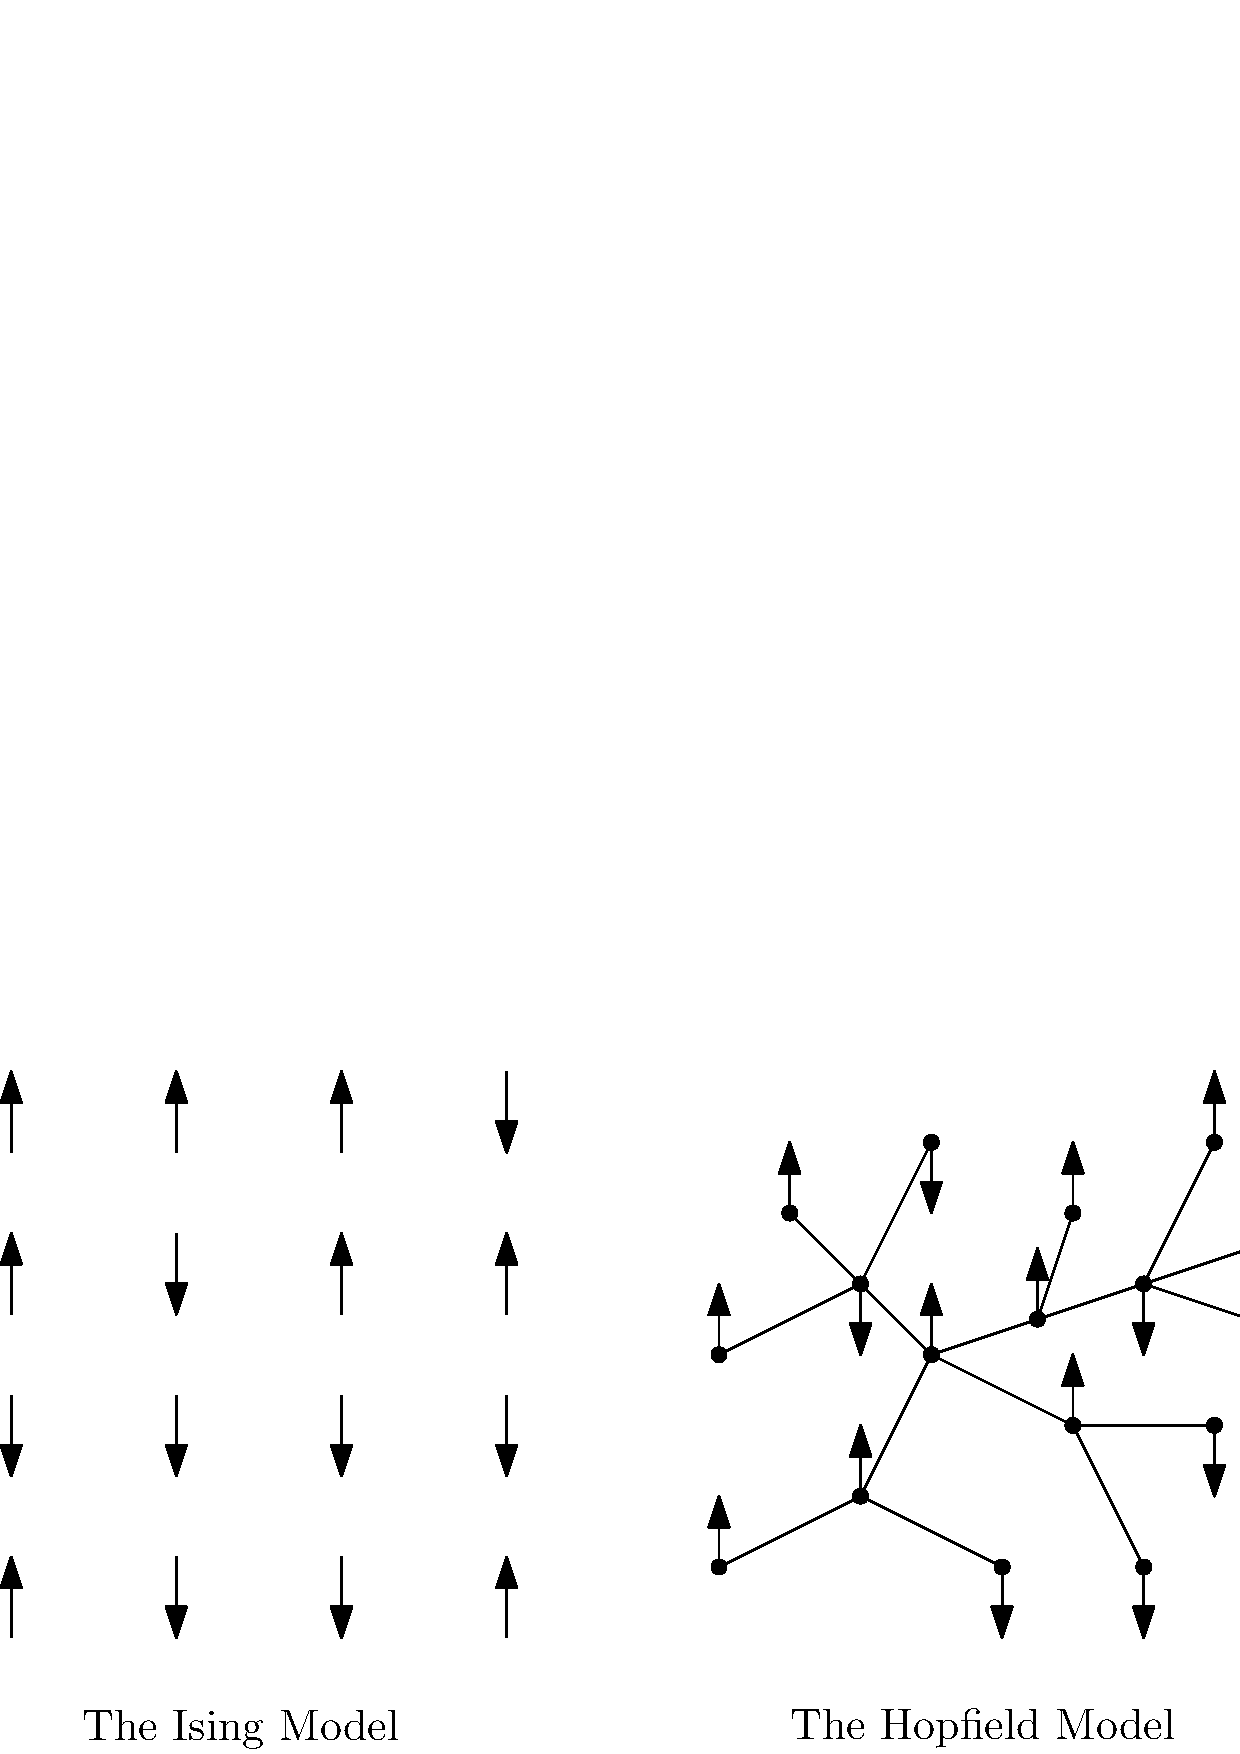
\includegraphics[width=\textwidth]{figures/evolution-anns.pdf}
  \caption{Restricted Boltzmann machines are a binary-valued two-layer
    neural network. RBMs trace their origins to the Hopfield model, an
    early model for associative memory which itself was inspired by
    the Ising model~\cite{hopfield}.\label{fig:rbm} }
\end{figure}

A full review of the techniques available in ML is beyond the scope of
this capstone. As such, we will focus our attention on one particular
class of algorithms, restricted Boltzmann machines (RBMs),
bidirectional artificial neural networks for modeling probability
distributions.  Depicted in \fref{fig:rbm}, RBMs consist of two layers
of binary units: a \textit{visible} layer,
${\bv}\eqcolon{\setv}_{i=0}^N$, and a \textit{hidden} layer,
$\bh\eqcolon\seth_{j=0}^N$, where $v_i,h_j\in\{0,1\}$. The visible
layer will serve as the input for our data, $\bx\rightarrow\bv$, and
the hidden layer as our prediction, $\bh\rightarrow\by$, the
label. For the purposes of classifying the phases of the 2D Ising
model, it will suffice to consider an RBM with one hidden unit,
$h$. If $h$ is $1$, we predict that the configuration is in the
ordered phase, and for $h=0$, we predict disordered. From our
exploration in the previous chapter, we could probably come up with
some function that performs this prediction. For example, we might sum
all of the spins (compute the magnetization), and if the result is
close to $0$ we know the system is disordered: $h:=0$. Otherwise, we would output $h\eqcolon 0$. The power of ML
will be to extract rules like these without explicit instructions.

Instead, we teach our model implicitly through the cost function,
$\mc{C}(P_{\theta}(y\rvert\bx), \{\mcX_{data}, \mcY_{data}\})$. This
acts as a moderator, and it tells the model how ``incorrect'' its
predictions (labels) are.  Formally, the ML goal becomes to find the
parameters $\theta$ that minimize $\mc{C}$. Experience from physics
tells us that finding the ground state (global minima) can be really,
\textit{really} hard.  Instead, we use stochastic gradient descent
(SGD). For each $\theta$, we calculate $\partial_{\theta}\mc{C}$, with
which we implement the update rule:
\begin{equation}%
  \theta \rightarrow \theta - \eta \partial_\theta \mc{C},
\end{equation}%
where $\eta$ is the \textit{learning rate}. From calculus, we know that the
negative gradient of a function is the direction in which that
function decreases most rapidly. This update procedure, then, adjusts
our parameters so as to reduce the cost. Iterating this procedure, we
end up in a local minimum of the cost function \sref{fig:sgd}. In
practice, we calculate these gradients, not over the entire data set,
but over subsets, \textit{minibatches}. This means the gradients will
vary from iteration to iteration (hence, \textit{stochastic}). This is
both computationally faster and introduces noise (like temperature)
that improves the chances of escaping poor local minima.

\begin{figure}[ht]
  \centering \includegraphics[width=0.75\textwidth]{figures/sgd.png}
  \caption{Stochastic Gradient Descent (SGD). If we view the cost
    function as defining an ``energy'' landscape, SGD allows us to
    find local minima (stable or metastable) energy states. Image
    taken from~\cite{sgd}.\label{fig:sgd} }
\end{figure}

Now, if we can formulate an adequate prediction function,
$P(\bh\rvert\bv)$, for the RBM, we can improve it with SGD. The
crucial step is to define an energy function:\label{sec:rbm-energy}%
\begin{equation}%
  \boxed{E_\theta(\bv, \bh)\eqcolon-\sum_i a_iv_i -\sum_j b_jh_j-\sum_{ij} w_{ij}v_ih_j \label{eq:rbm-energy-fn}}
\end{equation}
where $\theta\eqcolon\{\{a_i\},\{b_j\},\{w_{ij}\}\}$. Then, we can
model the system's joint probability with a Boltzmann distribution:%
\begin{equation}%
  \boxed{P_\theta(\bv,\bh)\eqcolon\frac{1}{Z}e^{-E_\theta(\bv,\bh)},\tab
    Z\eqcolon\sum_{\bv',\bh'}e^{E_\theta(\bv', \bh')}\label{eq:rbm-joint-dist}}
\end{equation}%
We note that this is the exact same equation as our Ising model
(\ref{eq:boltzmann-distribution} and~\ref{eq:ising-energy}). Here,
$\{a_i\}$ and $\{b_j\}$ take the role of the external magnetic field
$B$, which now varies from site to site (hence the indices $i$ and
$j$). Then, $\{w_{ij}\}$ takes the role of $J$ varying from pair to
pair.

Naturally, we run into the same intractability issues. For large
enough networks, we cannot evaluate $Z$. Instead of calculating joint
distributions, we pull a trick similar to MFT and MCMC, considering
instead conditional and marginal distributions. Due to RBM's bipartite
structure these factor and are easy to evaluate. Explicitly, in the
case of a single hidden spin $h_j$, we get (with a bit of algebra):
\begin{align}%
  P(h_j\rvert\bv)&=\frac{P(h_j,\bv)}{P(\bv)}=\frac{(e^{-E(\bv,h_j)})/Z}{(\sum_{\bh'}e^{-E(\bv,\bh')})/Z}\\
                 &=\frac{e^{-h_j(\sum_i w_{ij}v_i+b_j)}}{1+e^{(\sum_i w_{ij}v_i+b_j)}}.
\end{align}%
This conditional probability is itself a Boltzmann distribution, but
over only two states (tractable!).  We get for the full system:
\begin{equation}
  \boxed{P_\theta(\bh|\bv)=\prod_{j=1}^M \frac{1}{1+e^{-h_j(\sum_i w_{ij} v_i +b_j )}}
  }\label{eq:v-to-h}
\end{equation}%
and similarly:
\begin{equation}
  \boxed{P_\theta(\bv|\bh)=\prod_{i=1}^N \frac{1}{1+e^{-v_i(\sum_j w_{ij} h_j + a_i )}}
  }\label{eq:h-to-v}
\end{equation}

All that remains is for us to choose an adequate cost-function, and we
can start training our RBMs. For the example of binary-classification,
an appropriate choice is the cross-entropy loss:%
\begin{equation}%
  \mc{C}(P_\theta(\by\rvert\bx), \{\mcX_{data}, \mcY_{data}\})=\sum_{\bx\in\mcX_{data}} \sum_{\by\in\{0,1\}} P_{true}(\by\rvert\bx)\log P_\theta(\by\rvert\bx),
  \label{eq:cross-entropy}
\end{equation}%
see \sref{sec:cross-entropy} for elaboration. Differentiating with
respect to $\theta$ and with some simple algebra, we get the training
rule:%
\begin{align}%
  \partial_{b_j} \mc{C}&=\sum_{\bx\in\mcX_{batch}} P_{true}(\by\rvert\bx) \big[1-P_\theta(\by\rvert\bx)\big]\left(h_j\right),\\
  \partial_{w_{ij}}\mc{C}&=\sum_{\bx\in\mcX_{batch}} P_{true}(\by\rvert\bx)\big[1-P_\theta(\by\rvert\bx)\big]\left(v_i h_j\right).
\end{align}%
We have all the necessary elements of a phase classifier: a dataset, a
model of $P(\by\rvert\bx)$, and a means to train this model. In the
next section, we will consider an example more relevant to the
statistical physicist: generating samples.

\section{Generative Modeling: Gibbs
  Sampling}\label{sec:rbm-generative-modeling}
In \fref{sec:mc-overview}, we considered how to use MCMC sampling to
estimate macroparameters and even critical exponents.  Here we will
consider an MCMC technique called \textit{Gibbs Sampling} which will
use RBMs to generate samples of $P(\bx)$.

Suppose we are given an already trained RBM\@. Gibbs sampling, like other
MCMC techniques, consists of a series of update steps. In one step, we
input some initial state, transform it into a hidden state using
$P_\theta(\bh\rvert\bv)$, and transform it back to a new visible state
using $P_\theta(\bv\rvert\bh)$. This process is imperfect, so the
output of one step will differ from the input. If we repeat this
process many times, then the distribution of the outputs will converge
to the equilibrium distribution $P_\theta(\bv)$.

This first requires $P_\theta(\bv)$ to be an appropriate model of
$P_{true}(\bv)$. To get to this point, we need to derive a marginal
distribution over $\bv$ from $P_\theta(\bv,\bh)$. Similar to the
conditional probabilities, the architecture of the RBM allows us to
perform the marginalization
$P_\theta(\bv)=\sum_{\bh}P_\theta(\bv,\bh)$ explicitly. If we write
$P_\theta(\bv)$ as a Boltzmann distribution with its own energy
$E_\theta(\bv)$,
\begin{equation}%
  P_\theta(\bv)=\sum_{\bh} P_\theta(\bv,\bh) \propto e^{-E_\theta(\bv)},
\end{equation}%
then we can express $E_\theta(\bv)$ in terms of $E_\theta(\bv,\bh)$
\sref{sec:marginal}:
\begin{equation}
  \boxed{
    E_\theta(\bv)=-\sum_i a_i v_i -\sum_j \log\left(1 + \exp{-\left(b_j + \sum_{i} v_i w_{ij}\right)}\right),
    \label{eq:rbm-marginal-energy-v}
  }
\end{equation}
and we can perform an analogous computation for the marginal
distribution over $\bh$ to get $P_\theta(h)$ as a Boltzmann
distribution in terms of energy, $E_\theta(h)$. As in the
classification example, we require a cost function, in this case, the
Kullback-Leibler divergence (KLD):%
\begin{equation}
  \mc{C}(P_\theta(\bx),\bx)=D_{KL}(P_{data}(\bx)||P_{\theta}(\bx))\eqcolon\sum_{x\in\mcX_{data}} P_{true}(\bx)\ln\left(\frac{P_{true}(\bx)}{P_{\theta}(\bx)}\right). \label{eq:kld}
\end{equation}
This is closely related to the cross-entropy, and, similarly, it is an
important information-theoretic quantity \sref{sec:kld} that provides
a notion of similarity for probability distributions. It is $0$ if and
only if the two distributions are equal:
\begin{equation}%
  D_{KL}(P_{true}(\bx)||P_{\theta}(\bx))=0\iff P_{true}(\bx)=P_{\theta}(\bx).
\end{equation}%

We claimed that this unsupervised, but in comparing $\mc{C}$ in \fref{eq:kld}
with \fref{eq:cross-entropy}, we might interpret $\bx$ as a kind of
label for itself. A more appropriate description is
\textit{self-supervised}. We emphasize this point because it has been
the source of misunderstanding. ML always requires the specification
of a cost function, and even in the absence of labels, the cost function
guides how the model learns which information is relevant and irrelevant.

If we differentiate the KLD with respect to $\theta$, then after a bit
of algebra, we get:%
\begin{align}%
  \partial_{a_i} D_{KL}&=\expect{v_i}_{true}-\expect{v_i}_\theta\\
  \partial_{b_j} D_{KL}&=\expect{h_j}_{true}-\expect{h_j}_\theta\\
  \partial_{w_{ij}} D_{KL}&=\expect{v_i h_j}_{true}-\expect{v_i h_j}_\theta
\end{align}%
where $\expect{\ldots}_{true}$ is an average over the true
distribution $P_{true}(\bv)$ and $\expect{\ldots}_{\theta}$ is an
average over the model distribution $P_{\theta}(\bv)$.

If you take away one thing from this capstone, let it be this: sums
and averages like these are hard. Naturally, we approximate. Wherever
$h_j$ shows up, we use $P(h_j|\bv)$, and for the expectations over
$P_{true}$, we calculate a Monte Carlo average over our dataset,
$\mc{X}_{data}$. The expectations over $P_\theta$ are trickier. Fortunately,
we can approximate them with Gibbs sampling, initializing with samples
from $\mc{X}_{data}$. Together, these approximations constitute the
\textit{contrastive-divergence} algorithm, see~\cite{hinton}. Having trained our RBM, we
can generate new samples and start calculating critical exponents.

RBMs trained in this way have applications other than generation.
Consider training these on black and white images: if we constrain the
number of hidden nodes to be less than the number of visible nodes,
then the hidden layer will learn a compact representation of the
input. We can even stack multiple RBMs on top of each other to form
\textit{deep Boltzmann machines} (DBMs). In DBMs, the hidden layer of
one RBM becomes the visible layer of the next. Trained with
contrastive divergence, each layer learns a progressively compacter
version of the input.  This should remind you of RG\@. In the next
section, we will make these similarities more exact. Ultimately, this
allows us to machine learn RG transformations.
